\section{Memristors Crossbar Array}\label{sec:crossbar}

Setting memristors in a crossbar array to perform analog matrix multiplication typically called Multiply and Accumulate because of the nature of Matrix Multiplication. Figure \ref{fig:crossbar} shows what a typical crossbar array looks like.

\begin{figure}[H]
  \centering
  \subfloat[Schematics]{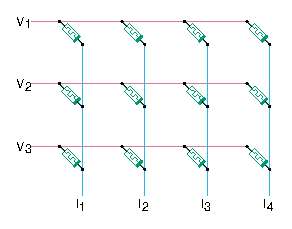
\includegraphics[width=.45\linewidth]{crossbar/crossbar.eps}}%\qquad
  \hfill
  \subfloat[3 dimensional representation]{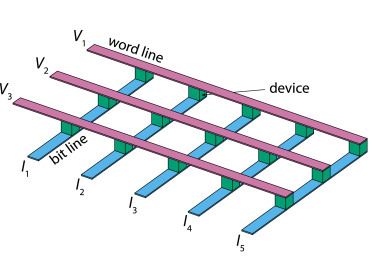
\includegraphics[width=.45\linewidth]{crossbar/crossbar3D.jpg}}\\
  \caption{Memristor crossbar array}
  \label{fig:crossbar}
\end{figure}

It uses physical properties of electrical systems to perform analog computing. Lets use the circuit node in figure \ref{fig:crossNode} to explain the theory behind the memristor crossbar array.
\begin{figure}[H]
  \centering
  \includesvg[height=3.5cm]{crossbar/crossbarNode.svg}
  \caption{Memristor crossbar node of the $i^{th}$ line and $j^{th}$ column}
  \label{fig:crossNode}
\end{figure}

First of all, a voltage is applied on the $i^{th}$ line, because every column is virtually grounded, the voltage applied to the memristor, of a set resistance of $R$, is $V_i$. As such and using Ohm's law, we know the the current flowing into the memristor is bound by the following equation :
\begin{equation}
  V_i = R\cdot I_{mem} \implies I_{mem} = V_i\cdot (\frac{1}{R})=I_{mem} = V_i\cdot G
\end{equation}
With $G$ being the conductance of memristor.
This line then joins the column where a current of $I_{i,j-1}$ is flowing, then according to kirchhoff's law the resulting current is :
\begin{equation}
  I_{j,i} = I_{j,i-1}+I_{mem} = I_{j,i-1} + V_i\cdot G
\end{equation}
By applying this process to the whole system we find that the current as the bottom of one column is :
\begin{equation}
  I_1=G_1\cdot V_1 + G_2\cdot V_2 + G_3\cdot V_3
\end{equation}
With $G_1$, $G_2$ and $G_3$ being the conductance of the 3 memristors in the first column.

This analog circuit removes the need to copy data from a main memory as the memristors themselves hold the value and the weights are then stored where the computation happens.
